\documentclass[11pt,a4paper]{article}
\usepackage[T1]{fontenc}
\usepackage{lmodern,microtype}
\usepackage[margin=21mm,headheight=15pt,headsep=7mm,footskip=10mm]{geometry}
\usepackage{booktabs,tabularx,array,amsmath}
\usepackage[dvipsnames]{xcolor}
\usepackage{pgfplots}
\pgfplotsset{compat=1.18}
\usepackage{caption,fancyhdr,titlesec,enumitem}
\usepackage[hidelinks]{hyperref}
\definecolor{ink}{HTML}{19384C}
\definecolor{teal}{HTML}{187F83}
\definecolor{gold}{HTML}{B87928}
\hypersetup{pdftitle={GrowingNN: First Progress Report -- Experiments 000--009},pdfauthor={GrowingNN project}}
\pagestyle{fancy}\fancyhf{}
\fancyhead[L]{\small\textcolor{ink}{GrowingNN\enspace /\enspace PyTorch migration}}
\fancyhead[R]{\small Progress report 01}
\fancyfoot[L]{\small Experiments 000--009}
\fancyfoot[R]{\small\thepage\ / 7}
\renewcommand{\headrulewidth}{0.3pt}
\titleformat{\section}{\Large\bfseries\color{ink}}{\thesection}{0.6em}{}
\titleformat{\subsection}{\normalsize\bfseries\color{ink}}{}{0em}{}
\titlespacing*{\section}{0pt}{5pt}{10pt}
\titlespacing*{\subsection}{0pt}{10pt}{4pt}
\setlength{\parindent}{0pt}\setlength{\parskip}{6pt}
\setlength{\tabcolsep}{5pt}\renewcommand{\arraystretch}{1.16}
\captionsetup{font=small,labelfont=bf,skip=5pt}
\setlist{nosep,leftmargin=1.4em}
\newcommand{\ev}[1]{\textcolor{ink}{\small[#1]}}
\newcommand{\note}[1]{{\small\textit{#1}\par}}
\pgfplotsset{every axis/.append style={font=\small,axis line style={black!35},tick style={black!35},grid=major,grid style={black!9},legend style={draw=none,font=\small},width=\linewidth,height=52mm}}
\begin{document}

{\small\bfseries\color{teal} RESEARCH AND DEVELOPMENT\quad /\quad REPORT 01}
\vspace{4mm}
{\Huge\bfseries\color{ink} GrowingNN\\[2mm] From prototype to\\[2mm] a PyTorch library\par}
\vspace{3mm}
{\large First progress report: experiments 000--009\par}
{\small Prepared for committee review\quad\textbullet\quad 23 November 2026}
\vspace{4mm}

\section{Purpose and progress}
GrowingNN began with a promising idea: a neural network can learn its weights while also changing its own structure. The earlier version was written from scratch using NumPy and basic numerical operations. That work motivated the next stage, but a custom numerical implementation is a difficult foundation for a library intended for wider use.

We are therefore rebuilding GrowingNN step by step in PyTorch. The aim is to make the method easier for other researchers and users to adopt, integrate with familiar training tools, and apply to larger problems. This report reviews the first experimental foundation for that transition. The description of the earlier NumPy version is project background; the experiments reported here do not benchmark it against PyTorch.

\subsection{What the system does}
Training proceeds in generations. Each generation first updates the model weights using gradient descent. If the search rule permits it, the system then evaluates possible architecture changes on a simulation set and applies one selected change. The next generation trains the changed network. Monte Carlo Tree Search (MCTS) is the original search method; several alternatives are evaluated in this report. Search is skipped after the final generation so that the delivered structure has a subsequent training measurement.

\subsection{What this reporting stage established}
Experiments 000--004 improved the basic training process: recovery after graph changes, legal growth operations, candidate scoring, and learning-rate control. Experiments 005--006 examined search quality and exposed a budget-handling defect. Experiments 007--008 moved to CIFAR-10 and established a configuration that finished above 91\% official test accuracy on three seeds. Experiment 009 then tested unrestricted growth across three datasets and showed that this stronger result does not yet transfer to every search configuration.

The main achievement is a working experimental basis for the PyTorch library, with clearer defaults and identifiable failure modes. It is not yet evidence that architecture search outperforms a well-trained fixed network, or that the library is ready for general release.

\subsection{Scope and reading guide}
This first report includes retrospective background through experiment 009. Source records extend from July into November 2026; they are not all runs from a single calendar month. Experiments 010 onward are outside scope. References \ev{E000}--\ev{E009} identify the corresponding preserved experiment reports; the accompanying source register gives exact report, data, and runner paths.

\note{Accuracy is reported as a percentage; changes in accuracy are percentage points (pp). Training, validation, and official test results are kept separate. Means include all seeds in the stated group unless explicitly identified otherwise.}

\newpage
\section{Making growth stable and possible}
\subsection{Experiment 000: recover after a change, not after every generation}
The first study addressed an interaction between two controls. The learning rate determines the size of weight updates; the simulation scheduler decides when a flat training curve permits architecture search. A repeating learning-rate cycle could flatten the curve even when the network had not exhausted its ability to learn.

The revised schedule kept the target rate between changes and restarted warmup only after an architecture action. Twelve MNIST runs compared two slope thresholds, three warmup shapes, and two seeds. Each run used a 420-parameter starter and ten generations. The historical loop recorded 11 epochs per generation, rather than the configured ten. \ev{E000}

\begin{center}
\begin{tabular}{lrrr}\toprule
Warmup & Final train (\%) & Final validation (\%) & Actions/run\\\midrule
Cosine &72.73&78.69&5.25\\
Logistic &84.34&88.28&5.25\\
Exponential &71.10&80.70&6.50\\\bottomrule
\end{tabular}
\captionof{table}{Experiment 000: means over both thresholds and seeds (four runs per row). The best individual configuration, 3$^\circ$ with logistic warmup, averaged 93.64\% final validation over two seeds.}
\end{center}

Architecture changes still disturbed training. The first action was followed by a mean validation gain of 14.96 pp over the next generation; fifth-or-later actions averaged $-0.13$ pp. These windows include ordinary training and do not isolate the causal benefit of the mutation. The study also found an unevaluated final mutation in every run. Before experiment 001, the protocol was changed to record exactly the configured epochs, seed the random generators consistently, and avoid terminal search. \ev{E000,E001}

\subsection{Experiment 001: smaller starters need a usable growth path}
Eighteen runs tested three initial depths, three thresholds (2$^\circ$, 3$^\circ$, 4$^\circ$), and two seeds, with logistic recovery fixed. The 420-, 276-, and 76-parameter starters averaged 91.20\%, 82.32\%, and 48.94\% final validation, respectively. A smaller start did not automatically produce a better growing model. \ev{E001}

The graph inspection explained part of the difficulty: sequential convolution was enabled but never generated as a legal candidate. The thin networks could add residual branches, yet could not directly rebuild a missing sequential convolution. This was a limitation in the available growth operations, not simply evidence that small models cannot learn.

\subsection{Experiment 002: repair the operation before comparing layouts}
After allowing convolution insertion before flattening, a corrected 16-run grid compared four starters at fixed width and pooling, using four seeds and five generations of ten epochs. The one-convolution/two-linear starter had the strongest all-seed mean final validation, 70.51\%, compared with 54.59\% for the larger starter. Its best seed reached 83.97\%. The larger model's mean includes two early dropout collapses; excluding them would raise it to 82.75\%, but would conceal a real reliability problem. \ev{E002}

The next question therefore became how to choose useful growth without repeatedly selecting harmful regularization. These studies established that legal graph edits, initial topology, and search behavior have to be evaluated together.

\newpage
\section{Improving selection and learning-rate control}
\subsection{Experiment 003: scoring must be tested with valid actions}
The next study compared grading candidates by training accuracy or validation accuracy. Two MNIST starters and four seeds gave 16 runs per phase, each with five generations of ten epochs and a 120-second search budget. A second phase banned repeated sequential dropout along the same graph path. \ev{E003}

\begin{center}
\begin{tabular}{lrrr}\toprule
Phase & Validation grading & Training grading & All runs\\
 &\multicolumn{3}{c}{Mean final validation accuracy (\%)}\\\midrule
Before path ban &58.42&61.73&60.08\\
After path ban &68.90&57.91&63.41\\\bottomrule
\end{tabular}
\captionof{table}{Experiment 003: each grading mean pools eight runs (two starters, four seeds); the overall mean pools 16. The apparent scoring preference changes after correcting the action constraint.}
\end{center}

Before the ban, training-based grading looked slightly better when starters were pooled, but two medium-model seeds each stacked four dropouts and collapsed near 21\% validation. After the ban, validation-based grading was better on both starters. Total dropout actions fell from 18 to nine across the grids, while residual-convolution additions rose from 12 to 21.

The adopted direction was to retain validation grading and the same-path dropout ban. This does not eliminate all weak runs: dropout on different paths can still harm learning. It also does not show that validation grading is universally superior; it supports that choice under the corrected settings tested here.

\subsection{Experiment 004: separate long-term decay from local recovery}
A growing network needs both an overall training schedule and time to recover after a mutation. Experiment 004 combined these controls:
\[
\eta_t=\max\!\left(0.001,\;b(t)\,r(t)\right),
\]
where $b(t)$ is the global learning-rate schedule and $r(t)$ is logistic recovery after a structure change. Seven schedules were tested on the big MNIST starter with validation grading, three matched seeds, and 100 real training epochs per run. All 21 runs completed. \ev{E004}

\begin{center}
\begin{tabular}{lrr}\toprule
Schedule & Mean final validation (\%) & Seed range (\%)\\\midrule
Step decay + recovery &89.37&87.89--92.11\\
Exponential decay + recovery &88.66&86.69--90.76\\
Cosine decay + recovery &86.38&81.90--90.40\\
Recovery only &74.53&50.37--86.87\\
Custom high-rate cascade &15.40&10.57--25.07\\\bottomrule
\end{tabular}
\captionof{table}{Selected schedules from experiment 004; all three seeds are retained. The custom cascade used a much larger base rate, 1.0 down to 0.1.}
\end{center}

Step decay had the highest mean, while exponential decay was close and was carried forward as the working package. Recorded rate curves followed the intended design. The poor high-rate cascade showed why a correctly implemented schedule can still be unsuitable. These MNIST findings guided the next experiments; later CIFAR work required its own training recipe.

\newpage
\section{Testing search, and learning from an invalid comparison}
\subsection{Experiment 005: compare alternatives to MCTS}
With exponential decay and logistic recovery fixed, the study compared 13 search algorithms on two MNIST starters and five seeds: 130 completed runs. Each run used ten generations of ten epochs. Candidate scoring used 2,000 simulation images and 15 training epochs, with a nominal 120-second search budget. \ev{E005}

\begin{center}
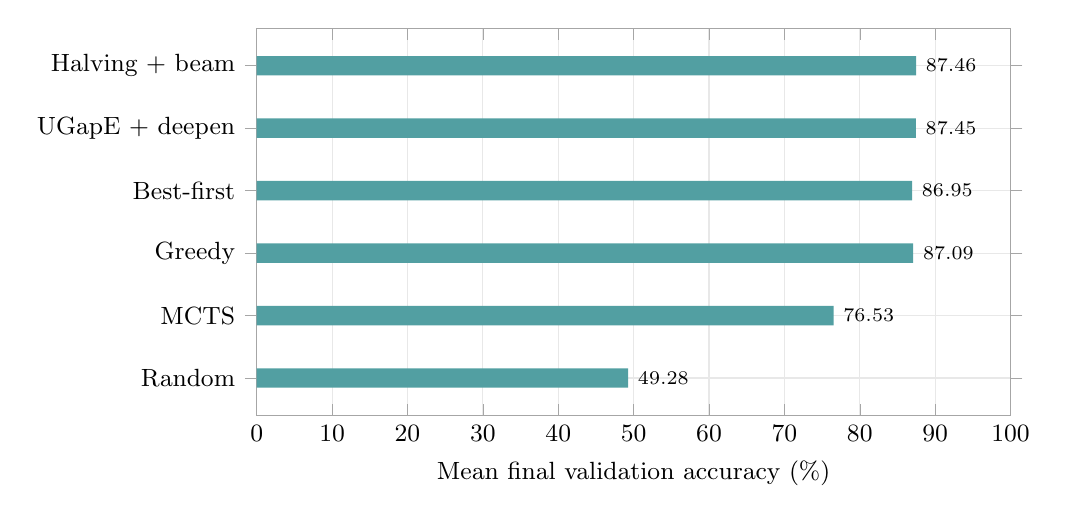
\begin{tikzpicture}
\begin{axis}[xbar,xmin=0,xmax=100,height=65mm,width=0.92\linewidth,
 xlabel={Mean final validation accuracy (\%)},
 symbolic y coords={Random,MCTS,Greedy,Best-first,UGapE + deepen,Halving + beam},
 ytick=data,nodes near coords,nodes near coords align={horizontal},
 nodes near coords style={font=\scriptsize},bar width=7pt,
 enlarge y limits=0.12]
\addplot[fill=teal!75,draw=none] coordinates {(49.28,Random) (76.53,MCTS) (87.09,Greedy) (86.95,Best-first) (87.45,UGapE + deepen) (87.46,Halving + beam)};
\end{axis}
\end{tikzpicture}
\captionof{figure}{Selected search methods from experiment 005. Each bar averages ten runs: five seeds on each of two starters. These are final validation scores, not official-test results.}
\end{center}

Sequential halving with beam search and UGapE with deepening reached the highest validation means among the selected methods. Best-first search also combined competitive accuracy with a small difference between starters. MCTS remained useful as a reference, but seed collapses lowered its mean. Random search provided a weak control.

Greedy search was nearly as strong as the leading methods. That limits what this task can establish about look-ahead: a good first action can dominate the result. The retained research set included halving with beam search, UGapE with deepening, best-first, and beam search, together with MCTS, greedy, and random controls. There was no basis to declare one method a universal default.

The nominal time limit also did not make computational work identical. MCTS performed extra training during expansion and rollout in addition to shared candidate scoring. Accuracy differences must therefore be read alongside differences in search execution, rather than as a pure comparison of decision rules.

\subsection{Experiment 006: a completed grid can still be inconclusive}
Twelve runs tested neuron addition/deletion ratios with halving-beam search, the big MNIST starter, and three seeds. The first pass over candidates exhausted the time budget before halving began. The shortlist then followed candidate generation order rather than the best scores, favoring residual convolution. A patch sorted candidates and required minimum halving rounds, but the published grid mixes runs before and after that change. \ev{E006}

Only three neuron-addition actions were executed, and no neuron-deletion actions. The doubling variant was never executed. Consequently, this experiment cannot justify enabling or disabling neuron resizing. Its useful contribution was the defect diagnosis and the requirement for a clean rerun with recorded candidate coverage and actual search cost.

\newpage
\section{Moving to a harder problem: CIFAR-10}
\subsection{Experiment 007: a stronger package, with a separate finish stage}
MNIST was useful for debugging, but could not establish readiness for more demanding image tasks. Experiment 007 compared the original CIFAR-10 recipe with a revised package on seeds 110--112. Both used a 45,000/5,000 training/validation split, crop-and-flip augmentation, and the separate official test set of 10,000 images. Search did not read the official test set. \ev{E007}

The original model began with 12,832 parameters, no starter BatchNorm, and 80 training epochs. The revised model began with 48,448 parameters and BatchNorm, inserted sequential convolutions before global pooling, and used a higher growth learning rate and gradient clipping. It trained for 56 growth epochs followed by 120 finish epochs with a fixed architecture. These are comparisons of complete packages with different budgets, not a single-change ablation.

\begin{center}
\begin{tabular}{lrrrr}\toprule
Seed & Original final & Revised growth & Best finish & Last finish\\
 &\multicolumn{4}{c}{Official CIFAR-10 test accuracy (\%)}\\\midrule
110 &72.79&82.16&90.19&89.98\\
111 &63.37&81.44&89.65&89.41\\
112 &64.20&82.38&89.84&89.66\\\midrule
Mean &66.79&81.99&89.89&89.68\\\bottomrule
\end{tabular}
\captionof{table}{Experiment 007: the original three-seed checkpoint comparison. ``Best finish'' selects the highest official-test measurement among 24 finish chunks; it is distinct from the final checkpoint.}
\end{center}

Only one best checkpoint crossed 90\%; none of the final checkpoints did. Selecting a peak using official-test measurements makes the best-finish column descriptive rather than an untouched estimate of final performance. The final mean of 89.68\% is the clearer endpoint. A later seed-110 history in the source is a different run, peaking at 89.93\%, and is not substituted for the original checkpoint result.

\subsection{Experiment 008: understand the plateau before extending training}
The broader CIFAR investigation explains why the package changed. An early augmented run spent 1,000 epochs training and ended at 66.44\% training and 67.28\% official test. Without live augmentation, a related run reached 97.95\% training but only 44.59\% test. Fitting the training images more closely had exposed overfitting. \ev{E008}

A larger comparison across four action groups and three seeds per group confirmed the value of augmentation. The 12 augmented runs averaged 72.56\% training and 76.96\% final test; the 12 unaugmented runs averaged 96.79\% training and 65.62\% test. Changing augmented views makes training accuracy harder to interpret in isolation.

Other diagnostics examined fixed image views, search algorithms, simulation scores, candidate training budgets, and conventional retraining of grown graphs. They did not identify search alone as the explanation. A longer improved run still plateaued near 86\% after 2,000 epochs. The evidence redirected work toward the interaction of the starter, convolution placement, normalization, and learning-rate behavior. Early studies sometimes used official-test data in candidate grading; those results form a development history, not a clean held-out benchmark.

\newpage
\section{Sustained learning within the generation loop}
Experiment 008 established the clearest reference without a separate finish stage. A larger BatchNorm starter, sequential-convolution additions, augmentation and random erasing, clipping, label smoothing, momentum 0.9, and a global cosine rate from 0.1 to 0.001 were used across 12 generations of ten epochs. Training, validation, and official test were separated into 45,000, 5,000, and 10,000 images. \ev{E008}

\begin{center}
\begin{tikzpicture}
\begin{axis}[height=64mm,xmin=10,xmax=120,ymin=50,ymax=100,
 xlabel={Real training epoch},ylabel={Official test accuracy (\%)},
 xtick={10,20,40,60,80,100,120},legend pos=south east]
\addplot[ink,thick,mark=*,mark size=1.4pt] table[x=epoch,y=seed110,col sep=comma]{data/experiment008_test.csv};
\addlegendentry{Seed 110}
\addplot[teal,thick,mark=square*,mark size=1.4pt] table[x=epoch,y=seed111,col sep=comma]{data/experiment008_test.csv};
\addlegendentry{Seed 111}
\addplot[gold,thick,mark=triangle*,mark size=1.6pt] table[x=epoch,y=seed112,col sep=comma]{data/experiment008_test.csv};
\addlegendentry{Seed 112}
\addplot[black!45,dashed,forget plot] coordinates {(10,90)(120,90)};
\end{axis}
\end{tikzpicture}
\captionof{figure}{Experiment 008 sequential-convolution reference: every recorded generation-end test measurement from the preserved snapshot. All seeds pass 90\% by epoch 100 and finish above 91\%. Lines connect measured points.}
\end{center}

The final official tests were 91.11\%, 91.17\%, and 91.36\%: a mean of 91.21\% and a range of 0.25 pp. Mean final training was 96.45\% and validation was 91.21\%. The graph grew from 187,008 to 1,813,248 parameters. Immediate validation changes at insertions were at most 0.08 pp; the substantial gains appeared during subsequent training. This is evidence that the changed network could keep learning, rather than evidence that an untrained inserted layer instantly improved accuracy.

\subsection{The success is real, but depends on the configuration}
Broader action sets remained less reliable. Under the initial generation-only comparison, all-action search averaged 85.68\% final test. A later 15-generation all-action configuration averaged 90.04\% across three seeds, but a nominally matching five-seed repeat with both training and convolution updates averaged 88.04\%. Wall-clock search limits can change candidate coverage and the resulting growth path even under the same nominal seed and settings. \ev{E008}

\begin{center}
\begin{tabular}{llr}\toprule
Learning-rate package & Convolution package & Mean final test (\%)\\\midrule
Old & Old &82.17\\
New & Old &83.23\\
Old & New &83.33\\
New & New &88.04\\\bottomrule
\end{tabular}
\captionof{table}{Experiment 008: five seeds per cell in the 15-generation all-action comparison. The new convolution package combines pre-pool placement, BatchNorm, and ReLU; their individual contributions are not separated.}
\end{center}

The combined changes improved the mean by 5.87 pp over the old package. This supports further development of the training-and-growth combination. It does not establish a matched-budget speedup over the early thousand-epoch run or an advantage over predetermined growth. Repeated inspection of official-test results also influenced development.

\newpage
\section{Broader validation and the next stage}
\subsection{Experiment 009: one general recipe, three datasets}
The final study in scope enabled every action and used seeds 1--3 on MNIST, CIFAR-10, and CIFAR-100. Each run trained for 20 generations of ten epochs, with a global cosine rate from 0.1 to 0.001. MCTS received eight seconds, one simulated epoch, and 128 simulation images. Starter sizes were 152, 187,008, and 268,672 parameters, respectively. \ev{E009}

\begin{center}
\begin{tabular}{lrrrr}\toprule
Dataset & Seed 1 & Seed 2 & Seed 3 & Mean\\
 &\multicolumn{4}{c}{Final official test accuracy (\%)}\\\midrule
MNIST &96.77&98.09&93.99&96.28\\
CIFAR-10 &86.25&86.04&86.82&86.37\\
CIFAR-100 &68.26&66.02&54.00&62.76\\\bottomrule
\end{tabular}
\captionof{table}{Experiment 009: all nine runs, with no seed exclusions. The active evidence set is \texttt{exp009\_small\_20}, not the older snapshot also named ``best reference''.}
\end{center}

CIFAR-10 was consistent across seeds, but its mean was 4.84 pp below the restricted-growth reference. It selected residual linear additions in 26 of 57 actions and sequential convolution only once. CIFAR-100 was less reliable: the weakest seed ended at 54.00\%, with a wide residual-linear structure, while the other seeds added more convolutions. MNIST showed that a very small starter could grow to useful accuracy, though its seed range was still 4.10 pp.

Final parameter counts were 5,793--9,016 on MNIST, 1.53--2.18 million on CIFAR-10, and 1.83--3.86 million on CIFAR-100. The saved graphs in the source are action-list replays, not recovered trained modules; some normalization and dropout details are ambiguous. The report therefore does not treat those drawings as exact checkpoint evidence.

\subsection{Assessment for the committee}
The migration has progressed from implementing growth to diagnosing when growth helps learning. The work produced protocol corrections, more usable convolution operations, an evidence-based scoring choice, composed learning-rate controls, a search comparison, and a stronger CIFAR training reference. The main limitation is now the reliability of selecting useful changes across tasks and seeds. More generations, more actions, or more simulation work did not consistently produce a better model.

For a user-oriented library, these results support documented configurations and reproducible experiment records. They do not yet demonstrate ease of installation, API usability, broader adoption, or performance at large scale. Those remain explicit delivery goals alongside the research work.

\subsection{Priorities for the next reporting period}
\begin{enumerate}
\item Compare searched growth, predetermined convolution growth, and fixed networks under matched training and compute budgets; choose checkpoints on validation and reserve test evaluation for the final comparison.
\item Rerun neuron resizing with one fixed search implementation, logging actual time, candidate coverage, and seed variation. Evaluate action gains separately by dataset and growth stage.
\item Preserve trained checkpoints, full histories, configurations, and code versions; turn the supported settings into simple examples and documented library entry points.
\end{enumerate}

\vfill
{\footnotesize\textbf{Evidence register.} [E000] scheduling; [E001] starter depth; [E002] topology; [E003] grading; [E004] composed rates; [E005] search methods; [E006] neuron resizing; [E007] CIFAR package; [E008] CIFAR development and generation-only studies; [E009] three-dataset growth. Sources are the experiment-000 through experiment-009 pages under \texttt{documentation/website/content/experiments/}, with data under \texttt{documentation/website/data/experiments/}. Exact filenames, runner paths, hashes, and chart provenance are recorded in the accompanying \texttt{SOURCES.md} and \texttt{source-manifest.json}.}
\end{document}
